\documentclass[Report.tex]{subfiles}

\newcommand{\baraxis}[8]{
\begin{axis}[
    ybar,
    title={#1},
    width=#5,
    height=#6,
    ymin=#3, ymax=#4,
    bar width=1em,
    legend style={at={#7},anchor=north,legend columns=-1},
    enlarge x limits=0.4,
    x tick label style={align=center,text width=#8},
    symbolic x coords={Logistic Regression, Random Forest, Multi-layer Perceptron},
    xtick=data,
    ylabel={#2}
]
}
% #1 - Number of splits
% #2 - Split number
% #3 - Feature name
% #4 - Column name
% #5 - Column legend name
\newcommand{\plotbar}[5]{
\addplot+[
	discard if not={numSplits}{#1},
	discard if not={split}{#2},
	discard if not={features}{#3},
] table [x=model, y=#4,col sep=comma] {data/19-pair-cv.csv};
\addlegendentry{#5}
}


% #1 - Title
% #2 - Y axis label
% #3 - Legend position
\newcommand{\lineaxis}[5]{
\begin{axis}[
    title={#1},
    grid=major,
    xmax=5, xmin=1,
    width=#3,
    height=#4,
%    ymin=0, ymax=1,
%    bar width=1em,
    legend style={at={#5},anchor=north,legend columns=-1},
    enlarge x limits=0.4,
	xlabel={Portion of match},
    ylabel={#2}
]
}


% #1 - ML model
% #2 - Feature name
% #3 - Metric name
% #4 - Legend name
\newcommand{\plotline}[4]{
\addplot+[
	discard if not={numSplits}{5},
	discard if not={model}{#1},
	discard if not={features}{#2}
] table [x=split, y=#3, col sep=comma] {data/19-pair-cv.csv};
\addlegendentry{#4}
}


\begin{document}



\section{Same player identification}\label{sec:pair-classification}
This sections describes the experiments and analysis of the second question: \textit{Given two matches of Dota 2, is it the same player playing on this hero?}

As the question has changed, some parts of the approach for player identification have changed to adapt to the new problem. Most notably, the mouse movement features were transformed in order to satisfy the need to have two matches as input instead of just one. 

\subsection{Approach}
%There was a subtle issue with the way the binary classification problem was framed in regards to classifying individual games. This led to high accuracies even with only using mouse movement features, as seen in section \ref{sbsec:game-classification}. The issue had to do with the generality of the model. The models were only trained on a relatively small, fixed set of players, making the problem easier to solve as the models only have to learn the behaviour from the players in the set, which does not apply(TODO) to the general Dota 2 playerbase. Furthermore, the classification is only trained on one particular playing and requires the model to be retrained to be able to predict behaviour of another player. This could be extended into a multi-class problem, but it would still be fixed to the small set of players used in training. This leads to the next machine learning approach of \textit{pair} classification.
%In the next and final approach, deals with this issue by framing the player prediction problem in a different way. Rather than ask \textit{Given a game, which player does it belong to?} the problem is framed as \textit{Given a pair of games, do both games belong to the same player?}
% TODO this leads to low testing accuracies?
% TODO results on a lot more players leads to worse accuracy

The goal of this approach was to be able to train on a large mix of players and games, to learn on features of both matches, and predict if it is the same player, especially if none of the players have been seen by the model before. Instead of learning to match behaviour to specific players, the idea becomes learning the pattern or differences in behaviour between two different players. 

In order to train on pairs of matches together, the input features had to be altered to fit as single data points. In the previous experiment, each match was evaluated separately, so every single mouse action in a game could be used and combined, as explained in section \ref{sec:game-approach}. However, in this pair approach, two matches must be used together as the input to a model. Matches in general are of different lengths, which causes the number of mouse actions to be different for every game. Further, the method of generating each mouse movement means even games of the exact same length will not have the same number of actions. The varying number of mouse actions prevents a straightforward use of them as input to a machine learning model. Instead, statistics such as the mean, standard deviation and range must be used. The statistics are calculated for each mouse movement feature over the entire match. For example, the horizontal velocity of a mouse action creates four features, the mean, standard deviation, minimum and maximum horizontal velocity of each \textit{individual} mouse action. There are numerous mouse actions in every match so further statistics of the four statistical features were created, giving new features such as the mean of the mean horizontal velocities. 

\begin{table}[H]
\centering
\begin{tabular}{| c | c | c | c |}
\hline
\textbf{Original property} & \textbf{Original features} & \textbf{New features} & \textbf{Number of features} \\ \hline
Angle of movement & \multirow{9}{3cm}{Minimum, maximum, mean, standard deviation} & \multirow{11}{3cm}{Minimum, 25\%, 50\%, 75\%, maximum, mean, standard deviation} & \multirow{9}{*}{$ 9 \times 4 \times 7 = 252 $} \\ \cline{1-1}
Curvature &  &  &  \\ \cline{1-1}
Rate of change of curvature &  &  &  \\ \cline{1-1}
Horizontal velocity &  &  &  \\ \cline{1-1}
Vertical velocity &  &  &  \\ \cline{1-1}
Velocity &  &  &  \\ \cline{1-1}
Acceleration &  &  &  \\ \cline{1-1}
Jerk &  &  &  \\\cline{1-1}
Angular velocity & & & \\ \cline{1-2} \cline{4-4}
Game ticks to command & \multirow{2}{*}{Single value} & & \multirow{2}{*}{$ 2  \times 7 = 14 $} \\ \cline{1-1}
Distance to command & & & \\ \hline
\end{tabular}
\caption{New features created after pre-processing mouse movement features for pair classification.}
\end{table}

This approach has many drawbacks. The most obvious is the loss of data from taking averages of averages, as the thousands of mouse actions are reduced to only a small number of statistics. To alleviate this issue as much as possible, the matches can be split into a few portions where each portion has its own statistics. For example, a match can be split into thirds where each third has its own mean and standard deviation for each mouse movement feature. Splitting a game this way not only decreases the data loss due to averaging, but enables each portion to be evaluated individually, to see whether any section of a game is more indicative and predictive of player behaviour compared to another section. The drawback with splitting matches like this was the large number of features that were created, leading to the curse of dimensionality and excessive computational requirements in extreme cases. Continuing with the horizontal velocity example, the original 4 features of minimum, maximum, mean and standard deviation are already transformed into 28 features. If a match is split in half and the features calculated for each half, then 56 features are created. Splitting a match into fifths will create 140 features for each property in the mouse movement actions. This disadvantage represents an interesting trade off between getting more fine-grained data and the curse of dimensionality. 

\subsection{Experimental design}
The experimental design for these experiments follow largely from the design described in section \ref{sec:game-experimental}, with a few key differences:
\begin{itemize}
\item For mouse movement features, each pair of matches could be split into different slices. This creates more features when used together, as a match split into two slices will have double the features, one set for each half of the match. This also allowed for comparisons to be made for each slice, to see if any portion of a match is more predictive than another. 
\item A modified dataset was created for this set of experiments. The dataset was created in order to prevent data leakage, as the original contained one player which appeared in both the training and testing sets, which made sense in the previous problem. The number of data points in the new modified dataset also changed due to the nature of the inputs for each problem. Here, the new dataset was created by taking a combination of every pair of matches, so many more samples can be created with fewer matches. Moreover, no single player belonged to a majority of matches, to prevent models becoming biased towards learning only a particular player's behaviour.

\end{itemize}


\subsubsection{Dataset information}
For the modified dataset less players were used with more matches each to create as many positive samples (two matches from the same player) as possible. This resulted in 38 players total with 218 a total of replays, about 5-6 replays for each player. In terms of positive and negative samples after creating combinations of pairs of matches, there was a total of 2970 positive samples and 3071 negative samples. The number of negative samples was significantly reduced in order to balance the two classes. A majority number of samples in one class would affect the performance of machine learning models as a model can become biased towards the majority class, since predicting that class will give increased accuracy due to the nature of the dataset. For this reason, many negative samples were removed.

\subsection{Mouse movement features}

\begin{figure}[H]
\centering
\begin{tikzpicture}
\baraxis{\textbf{Classification with mouse movement features}}{Metric rate}{0.3}{1.03}{9cm}{5cm}{(0.5,-0.45)}{1.7cm}

\plotbar{1}{1}{mouse}{accuracy}{Accuracy}
\plotbar{1}{1}{mouse}{precision}{Precision}
\plotbar{1}{1}{mouse}{recall}{Recall}

\end{axis}
\end{tikzpicture}
\caption{Accuracy, precision and recall of using mouse movement features only when classifying a pair of matches.}
\end{figure}

Looking at mouse movement features only, it can be seen the the logistic regression model performs poorly compared to the other two models. There are two likely explanations for this. The first is because logistic regression typically assumes some form of linear relationship between the input and output. As the mouse movement features were not transformed in such a way to better uncover a linear relationship to the output, the non-linear based algorithms of random forest and multi-layer perceptron were better able to distinguish and predict whether the two input matches were from the same player. The second reason why logistic regression may have performed poorly is due to the increased number of features relative to the number of data points available in training. In a comparison of logistic regression to other classifiers, Yoo et al. \cite{lr-vs-rf} demonstrated that logistic regression performed poorly when the number of features was greater than the number of sample data points. That was not the case here, as there were 268 features and a few thousand data points, but perhaps the ratio of features to data points played a role. It is difficult to pinpoint the exact reason, and although further analysis of the other features hints towards the first reason.

In a rudimentary comparison to the previous experiment, the results were weaker across the board here. No metric got over 80\% where both logistic regression and multi-layer perceptron models got over 80\% for just mouse movement. This could be attributed to two causes, the loss of data from averaging and the increased difficulty of the problem. The difference in the two datasets makes the comparison difficult, as this dataset creates more data points and has a more diverse number of players. 

% It shall be shown when investigating the other features that the loss of data from averaging was not the root cause. The other features such as itemisation did not have the drawback of averaging but similarly performed worse compared to the previous experiment. 
\begin{figure}[H]
\begin{subfigure}{1\textwidth}
\centering
\begin{tikzpicture}
\baraxis{\textbf{Accuracy of different slices}}{Accuracy rate}{0.3}{1}{9cm}{5cm}{(0.5,-0.45)}{1.7cm}

\plotbar{1}{1}{mouse}{accuracy}{1 slice}
\plotbar{2}{2}{mouse}{accuracy}{2 slices}
\plotbar{3}{3}{mouse}{accuracy}{3 slices}
\plotbar{5}{5}{mouse}{accuracy}{5 slices}

\end{axis}
\end{tikzpicture}
\end{subfigure}

\begin{subfigure}{0.45\textwidth}
\centering
\begin{tikzpicture}[scale=0.75]
\baraxis{\textbf{Precision of different slices}}{Precision rate}{0.3}{1}{9cm}{5cm}{(0.5,-0.45)}{1.7cm}

\plotbar{1}{1}{mouse}{precision}{1 slice}
\plotbar{2}{2}{mouse}{precision}{2 slices}
\plotbar{3}{3}{mouse}{precision}{3 slices}
\plotbar{5}{5}{mouse}{precision}{5 slices}
\legend{};
\end{axis}
\end{tikzpicture}
\end{subfigure}
\hspace{\fill}
\begin{subfigure}{0.45\textwidth}
\centering
\begin{tikzpicture}[scale=0.75]
\baraxis{\textbf{Recall of different slices}}{Recall rate}{0.3}{1}{9cm}{5cm}{(0.5,-0.45)}{1.7cm}

\plotbar{1}{1}{mouse}{recall}{1 slice}
\plotbar{2}{2}{mouse}{recall}{2 slices}
\plotbar{3}{3}{mouse}{recall}{3 slices}
\plotbar{5}{5}{mouse}{recall}{5 slices}
\legend{};
\end{axis}
\end{tikzpicture}
\end{subfigure}
\caption{Metric scores with mouse movement features when a match is split into a different number of portions and they are used together. Note that more slices means a greater number of features, as the featureset is repeated for each slice.}
\end{figure}

When splitting a match into multiple portions and using all portions together in training, the poor performance of logistic regression can again be seen clearly underperforming compared to the other two models. However, a key point of interest is how there is no significant decline in accuracy as the number of splits increases, which one would expect if Yoo et al.'s \cite{lr-vs-rf} findings were to be confirmed, as the difference between 1 split and 5 splits is five times the number of features. The accuracy does fall for 2 splits, but grows again for 3 and 5 splits. This suggests a more complicated reason than simply logistic regression performing poorly because the number of features was too large, likely showing the linear model reaching it's limitations. Nevertheless, the random forest and multi-layer perceptron shows loss of accuracy as more slices are used together, with the random forest showing the highest loss, from 85\% to 76\%. This shows the additional slices likely add too many features and introduce noise as uncorrelated patterns are drawn, for example mouse movement data from the first slice of one game with the mouse movement data from the third slice of the other game. 

% random forest getting less accuracy with more splits, too many features adds too much noise?

Next, instead of concatenating the sections of a match together, each individual slice was tested.

\begin{figure}[H]
\centering
\begin{tikzpicture}
\lineaxis{Accuracy for different portions of a match}{Accuracy rate}{12cm}{6cm}{(0.5,-0.25)}

\plotline{Logistic Regression}{mouse}{accuracy}{Logistic Regression}
\plotline{Random Forest}{mouse}{accuracy}{Random Forest}
\plotline{Multi-layer Perceptron}{mouse}{accuracy}{Multi-layer Perceptron}

\end{axis}
\end{tikzpicture}
\caption{Metric scores with mouse movement features on individual portions of a match. }
\end{figure}

There were no significant results from using slices of a match individually, only small deviations from the accuracy when no slicing was done at all. This result is rather unexpected, as the strategy and gameplay in different phases of a Dota 2 game change, and naturally, one would assume the mouse movement behaviour of players change as well. A point to consider is that though the strategy and behaviour may change between the phases of a game, many players' behaviour change in the same way, so there is little change in the difference of behaviour \textit{between} two players. Further, the phases changes in a Dota 2 match usually happen at different times, depending on how much of an advantage one team is able to amass. 

%TODO 

\subsection{Game statistic features}
Next are the game statistic features. A slightly different trend can be seen compared to the mouse movement features. Logistic regression continues to perform poorly, but the multi-layer perceptron model interestingly has very high recall but low accuracy and precision. This was the inverse of the pattern observed when looking at single matches in section \ref{sbsec:game-classification}, where the random forest classifier obtained high precision but low recall. The two patterns are likely unrelated, as they occurred on different classification problems, featuresets and models.

% More on same pattern TODO

\begin{figure}[H]
\centering
\begin{tikzpicture}
\baraxis{\textbf{Metrics for classifying pairs of games with game statistic features}}{Metric rate}{0.3}{1.03}{9cm}{6cm}{(0.5,-0.35)}{1.7cm}

\plotbar{1}{1}{stats}{accuracy}{Accuracy}
\plotbar{1}{1}{stats}{precision}{Precision}
\plotbar{1}{1}{stats}{recall}{Recall}

\end{axis}
\end{tikzpicture}
\caption{Accuracy, precision and recall rates using only game statistics such as gold and XP per minute when classifying a pair of matches.}
\end{figure}

The random forest classifier gave the best results with just game statistics by a large margin. This was somewhat expected, as it also performed the best in the previous experiment. It is interesting that the performance translated to this experiment very well. This shows a strong correlation between in game statistics and player prediction for random forest, both in identifying a particular player and in identifying the difference between two players. 

\begin{figure}[H]
\vspace{-2cm}
\begin{subfigure}{1\textwidth}
\image{0.9\textwidth}{imgs/correlation-stats0.png}{Correlation matrix for pairs by different players}
\end{subfigure}

\begin{subfigure}{1\textwidth}
\image{0.9\textwidth}{imgs/correlation-stats1.png}{Correlation matrix for pairs by the same players}
\end{subfigure}
\caption{Correlation matrices showing the statistics for one match of a pair against the other.}
\label{fig:stats-correlation}
\end{figure}

The correlation between the statistics of one match compared to the statistics of the other match in a pair can help give insight into which statistics are more impactful. Figure \ref{fig:stats-correlation} shows the correlation matrices between pairs by different players and pairs by the same players. The differences between the two matrices again show much higher correlation for pairs where both matches were by the same player. A small number of statistics are seen to be stronger indicators than others. First, the kills, deaths and assists (KDA) do not look well correlated. This was speculated earlier, as the KDA of players vary often in a small range. The gold and XP statistics are also better correlated between two matches by the same player when looking at per minute statistics instead of the absolute gold and XP earned by the end of a match. 

There are a few key points to notice for the gold and XP per minute statistics. The CS, denies, gold per minute, XP per minute and CS per minute scores are well correlated to each other even across different matches, as long as the player was the same. It would be expected for these numbers to be correlated in the same match, as creeps directly affect the gold and XP gained by heroes. However, seeing the statistics continue this trend across different matches suggest they are also tied to specific player behaviour. The same pattern can be seen for movement commands, and to a lesser extent the attack and spell cast commands. This is very interesting, and suggests using the statistics together gives better results that compared each individually across a pair. 

Finally, it should be noted that the correlation matrix for pairs of matches by the same players is mirrored across the diagonal. This is a result of the combination step, where matches are combined into pairs of \textit{\{match0, match1\}} and \textit{\{match1, match0\}} and should not be taken as a meaningful result.

Due to the way the \texttt{clarity} parser functions by running through matches chronologically, and a bug which prevents the library from seeking directly to a time or tick in a match, splitting up a match into equally sized portions on the go was not possible and so, detailed data about game statistics on different sections of a match could not be gathered.  

\subsection{Itemisation features}

For itemisation features, each encoding method is compared. On the whole, using only boots by themselves was the best indicator for random forest and multi-layer perceptron, while the item differences were best for the logistic regression model. Once again, logistic regression did not have good results compared to the random forest and multi-class perceptron models. The only exception is the item difference method of encoding, where it was able to get higher accuracies than the random forest and multi-layer perceptron models using the same feature. This is a bit of an anomaly, as the trend so far suggests logistic regression is not suitable for this classification task. 

The difference between the item difference feature and all other features used, including the game statistics and mouse movement features is that the features are not duplicated for the pair of matches. For all other features, the features for both matches are used together, as it may be interesting to see if different features across the two matches may be correlated. However for the item difference, the presence or absence of the same item on an inventory slot is encoded and so there is no duplication of features. This contrast is likely the reason for a reduction in complexity that allowed the logistic regression model to perform comparably to the other two models where all other features could not.

\begin{figure}[H]
\centering
\centering
\begin{tikzpicture}
\baraxis{\textbf{Accuracy with game itemisation features}}{Accuracy rate}{0.4}{1}{15cm}{4.5cm}{(0.5,-0.35)}{2cm}

\plotbar{1}{1}{items-hashed}{accuracy}{Hashed items}
\plotbar{1}{1}{items-onehot}{accuracy}{One-hot}
\plotbar{1}{1}{items-starting}{accuracy}{Starting items}
\plotbar{1}{1}{items-select}{accuracy}{Boots only}
\plotbar{1}{1}{items-diff}{accuracy}{Item differences}
\legend{};
\end{axis}
\end{tikzpicture}

\begin{tikzpicture}
\baraxis{\textbf{Precision with game itemisation features}}{Precision rate}{0.4}{1}{15cm}{4.5cm}{(0.5,-0.35)}{2cm}

\plotbar{1}{1}{items-hashed}{precision}{Hashed items}
\plotbar{1}{1}{items-onehot}{precision}{One-hot}
\plotbar{1}{1}{items-starting}{precision}{Starting items}
\plotbar{1}{1}{items-select}{precision}{Boots only}
\plotbar{1}{1}{items-diff}{precision}{Item differences}
\legend{}; % hide legend

\end{axis}
\end{tikzpicture}

\begin{tikzpicture}
\baraxis{\textbf{Recall with game itemisation features}}{Recall rate}{0.4}{1}{15cm}{4.5cm}{(0.5,-0.38)}{2cm}

\plotbar{1}{1}{items-hashed}{recall}{Hashed items}
\plotbar{1}{1}{items-onehot}{recall}{One-hot}
\plotbar{1}{1}{items-starting}{recall}{Starting items}
\plotbar{1}{1}{items-select}{recall}{Boots only}
\plotbar{1}{1}{items-diff}{recall}{Item differences}

\end{axis}
\end{tikzpicture}
\caption{Accuracy, precision and recall for different game itemisation encoding methods.}
\end{figure}

There are a few other notable results for the item encoding methods. Firstly, the hashed items was able to obtain accuracies higher than the one-hot encoded items for random forest, but not for the neural network. Moreover, the recall was relatively lower while the precision was higher in the random forest. 

Secondly, the one-hot encoding of all items performed very similarly to the one-hot encoding of only starting items. This was surprising because the one-hot encoding of all items contained 250 more items than the starting items, which translates to 1500 more binary features. This was also the case in the previous classification task and it continues to be the case here, that the increased number of binary features had little effect on the performance of the models. The gap between the two methods is smaller than previously, which means just using starting items to differentiate between two players is more difficult than identifying a single player. This may be because a more diverse pool of players here leads to more similarity in starting items between any two players. 

\subsection{Combined features}

\subsubsection{Comparison of feature individually}

\begin{figure}[H]
\newcommand{\comparisonaxis}[2]{
\begin{axis}[
	title={\textbf{#1}},
	ylabel={#2},
	ybar,
	bar width=1.5em,
	width=15cm,
	height=4cm,
	legend style={at={(0.5,-0.35)},anchor=north,/tikz/every even column/.append style={column sep=0.5cm}},
	xtick=data,
	enlarge x limits=0.25,
	ymin=0.4, ymax=1,
	symbolic x coords={Logistic Regression, Random Forest, Multi-layer Perceptron},
    x tick label style={align=center,text width=2.5cm},
]
}
\centering
\begin{tikzpicture}
\comparisonaxis{Accuracy of features individually}{Accuracy rate}

\plotbar{1}{1}{mouse}{accuracy}{Mouse movement only}
\plotbar{1}{1}{stats}{accuracy}{Game statistics only}
\plotbar{1}{1}{items-select}{accuracy}{Boots only}
\plotbar{1}{1}{items-diff}{accuracy}{Item difference}
\legend{};
\end{axis}
\end{tikzpicture}

\begin{tikzpicture}
\comparisonaxis{Precision of features individually}{Precision rate}

\plotbar{1}{1}{mouse}{precision}{Mouse movement only}
\plotbar{1}{1}{stats}{precision}{Game statistics only}
\plotbar{1}{1}{items-select}{precision}{Boots only}
\plotbar{1}{1}{items-diff}{precision}{Item difference}
\legend{};
\end{axis}
\end{tikzpicture}

\begin{tikzpicture}
\comparisonaxis{Recall of features individually}{Recall rate}

\plotbar{1}{1}{mouse}{recall}{Mouse movement only}
\plotbar{1}{1}{stats}{recall}{Game statistics only}
\plotbar{1}{1}{items-select}{recall}{Boots only}
\plotbar{1}{1}{items-diff}{recall}{Item difference}

\end{axis}
\end{tikzpicture}
\caption{Accuracy for pair classification with different features and models.}
\end{figure}


It can be concluded quite definitively from analysing the features individually that logistic regression was not well suited to this classification problem. In every feature, logistic regression struggled to get a 50\% classification rate, with only the boots only feature getting a 59\% correct classification. The only exception is the item difference feature, which was able to transform the complexity of the problem by calculating the difference and not duplicating the features. As such, there is a clear difference in the complexity of the classification problem compared to the previous experiment, where logistic regression was able to obtain strong results. It is also unlikely that Yoo et al.'s explanation of poor logistic regression performance with a large number of features \cite{lr-vs-rf} applies here, as the game statistic features had a small number of features while mouse movement had a large number of features. 

%TODO it would be interesting to see if other features, like game stats difference could also be calculated, and if lr would continue to work for that

There are a few model and feature combinations that stand out with the best individual performance. Random forest in general was able to obtain highest accuracies with all different features. The neural network had comparable results for the itemsation features, but not for the mouse movement or statistic features. This is interesting because the mouse movement and statistic features were the best performing features for the random forest classifier. This suggests there is no stand out best feature to determine if two matches come from the same player, but rather, different models are able to apply the different features with varying degrees of success. A similar conclusion was reached by Liu et al. \cite{starcraft-identification} for player identification in Starcraft 2. 

\subsubsection{Logistic regression}
As mentioned, logistic regression performed poorly overall in this classification task, with only the item difference feature working well due to its reduced complexity. The large majority of feature combinations without this feature did not achieve better predictions, so attention is drawn on the combinations of item difference and other features. 

\begin{figure}[H]
\centering
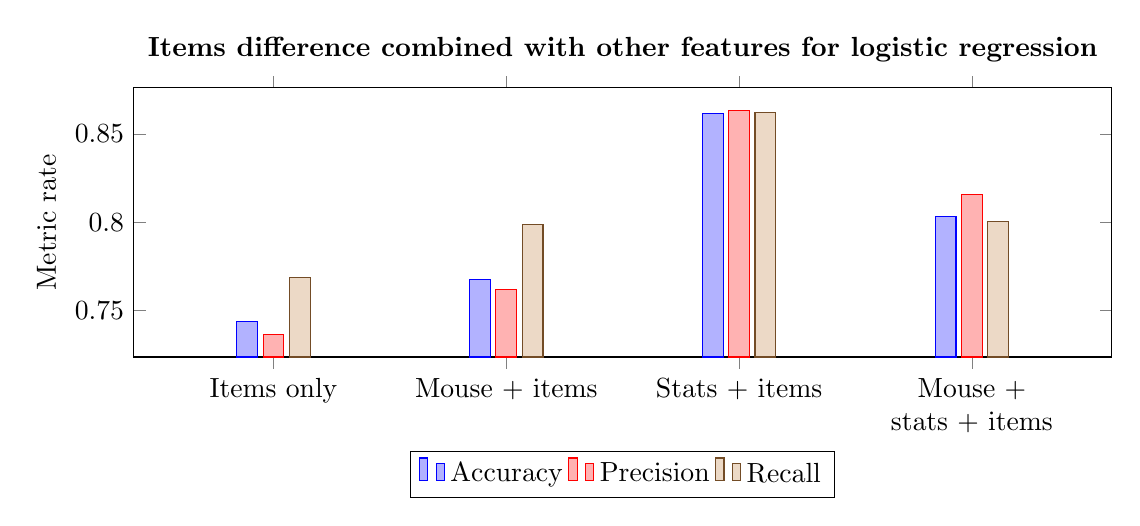
\begin{tikzpicture}
\begin{axis}[
    ybar,
    title={\textbf{Items difference combined with other features for logistic regression}},
    width=14cm,
    height=5cm,
    %ymin=0.4, ymax=1,
    bar width=0.75em,
    legend style={at={(0.5,-0.35)},anchor=north,legend columns=-1},
    enlarge x limits=0.2,
    x tick label style={align=center,text width=3cm},
    symbolic x coords={Items only, Mouse + items, Stats + items, Mouse + stats + items},
    xtick=data,
    ylabel={Metric rate},
    %cycle list name=exotic,
    %every axis plot/.append style={fill,draw=none,no markers}% <- added
]
\addplot table [x=features, y=accuracy, col sep=comma] {
numSplits,split,accuracy,precision,recall,model,features
1,1,0.7437536518359378,0.7362784744668971,0.7684284784024311,Logistic Regression,Items only
1,1,0.7672500046753832,0.762021495693811,0.7987112003472976,Logistic Regression,Mouse + items
1,1,0.8614543841197742,0.8633472815673985,0.862122856522683,Logistic Regression,Stats + items
1,1,0.8033406413964528,0.8157132392501388,0.8001220968092033,Logistic Regression,Mouse + stats + items
};
\addlegendentry{Accuracy}

\addplot table [x=features, y=precision, col sep=comma] {
numSplits,split,accuracy,precision,recall,model,features
1,1,0.7437536518359378,0.7362784744668971,0.7684284784024311,Logistic Regression,Items only
1,1,0.7672500046753832,0.762021495693811,0.7987112003472976,Logistic Regression,Mouse + items
1,1,0.8614543841197742,0.8633472815673985,0.862122856522683,Logistic Regression,Stats + items
1,1,0.8033406413964528,0.8157132392501388,0.8001220968092033,Logistic Regression,Mouse + stats + items
};
\addlegendentry{Precision}

\addplot table [x=features, y=recall, col sep=comma] {
numSplits,split,accuracy,precision,recall,model,features
1,1,0.7437536518359378,0.7362784744668971,0.7684284784024311,Logistic Regression,Items only
1,1,0.7672500046753832,0.762021495693811,0.7987112003472976,Logistic Regression,Mouse + items
1,1,0.8614543841197742,0.8633472815673985,0.862122856522683,Logistic Regression,Stats + items
1,1,0.8033406413964528,0.8157132392501388,0.8001220968092033,Logistic Regression,Mouse + stats + items
};
\addlegendentry{Recall}

\end{axis}
\end{tikzpicture}
\caption{The item difference encoding method combined with other features yielded good results for logistic regression, even when all other combinations of features did not. }
\end{figure}

The combination of other features with the item difference encoding was able to clearly boost the prediction rate of the logistic regression model. Recall that mouse movement and game statistic data alone could not even achieve a 50\% classification rate. The combination of other itemisation methods with mouse movement and game statistics also do not go above this 50\% classification rate except when using the game statistics and boots features together, which only gives 52\% accuracy. This may be related, as the combination of game statistics and the item difference is the best performing set of features for logistic regression. Further, there is a large difference between using mouse movements or using game statistics with the itemisation features, which is surprising given there was little difference between the two featuresets when they were evaluated individually. 

% All other mouse + stats + item combinedations also only about <50% classification

% No other combinations of features achieved anywhere near significant gains in performance

\subsubsection{Random forest}

The random forest classifier performed very consistently overall when using any of the featuresets by themselves. The combination of features was also able to further boost performance. Two noteworthy examples are presented. The first takes a look at how the performance of using boots data is altered as more features are added and the second looks into the improved performance as more features are added with starting items features. These results help shed light into the improvements in accuracy that can be made by using multiple features together.

\begin{figure}[H]
\centering
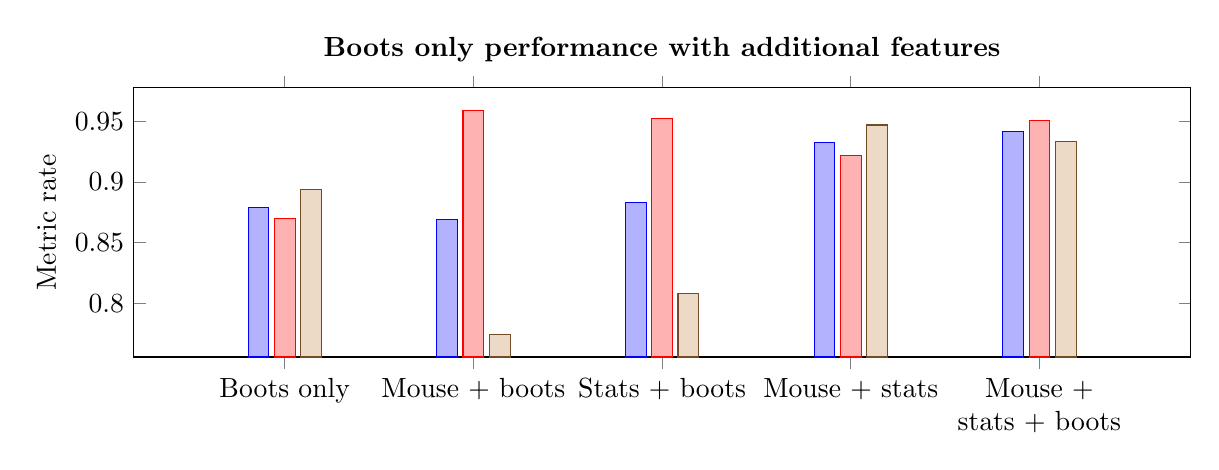
\begin{tikzpicture}
\begin{axis}[
    ybar,
    title={\textbf{Boots only performance with additional features}},
    width=15cm,
    height=5cm,
    %ymin=0.4, ymax=1,
    bar width=0.75em,
    legend style={at={(0.5,-0.35)},anchor=north,legend columns=-1},
    enlarge x limits=0.2,
    x tick label style={align=center,text width=2.5cm},
    symbolic x coords={Boots only, Mouse + boots, Stats + boots, Mouse + stats, Mouse + stats + boots},
    xtick=data,
    ylabel={Metric rate},
    %cycle list name=exotic,
    %every axis plot/.append style={fill,draw=none,no markers}% <- added
]
\addplot table [x=features, y=accuracy, col sep=comma] {
numSplits,split,accuracy,precision,recall,model,features
1,1,0.879328056504667,0.8700523463632187,0.8938056218797481,Random Forest,Boots only
1,1,0.868903225353162,0.9590398493485237,0.7743026915563274,Random Forest,Mouse + boots
1,1,0.8830309936062454,0.9520265857015682,0.8082021923160407,Random Forest,Stats + boots
1,1,0.9415068228048351,0.9504757706851802,0.9335874755806381,Random Forest,Mouse + stats + boots
1,1,0.9322103786068515,0.9219059921138925,0.9469068808335143,Random Forest,Mouse + stats

};

\addplot table [x=features, y=precision, col sep=comma] {
numSplits,split,accuracy,precision,recall,model,features
1,1,0.879328056504667,0.8700523463632187,0.8938056218797481,Random Forest,Boots only
1,1,0.868903225353162,0.9590398493485237,0.7743026915563274,Random Forest,Mouse + boots
1,1,0.8830309936062454,0.9520265857015682,0.8082021923160407,Random Forest,Stats + boots
1,1,0.9415068228048351,0.9504757706851802,0.9335874755806381,Random Forest,Mouse + stats + boots
1,1,0.9322103786068515,0.9219059921138925,0.9469068808335143,Random Forest,Mouse + stats
};

\addplot table [x=features, y=recall, col sep=comma] {
numSplits,split,accuracy,precision,recall,model,features
1,1,0.879328056504667,0.8700523463632187,0.8938056218797481,Random Forest,Boots only
1,1,0.868903225353162,0.9590398493485237,0.7743026915563274,Random Forest,Mouse + boots
1,1,0.8830309936062454,0.9520265857015682,0.8082021923160407,Random Forest,Stats + boots
1,1,0.9415068228048351,0.9504757706851802,0.9335874755806381,Random Forest,Mouse + stats + boots
1,1,0.9322103786068515,0.9219059921138925,0.9469068808335143,Random Forest,Mouse + stats
};

\end{axis}
\end{tikzpicture}

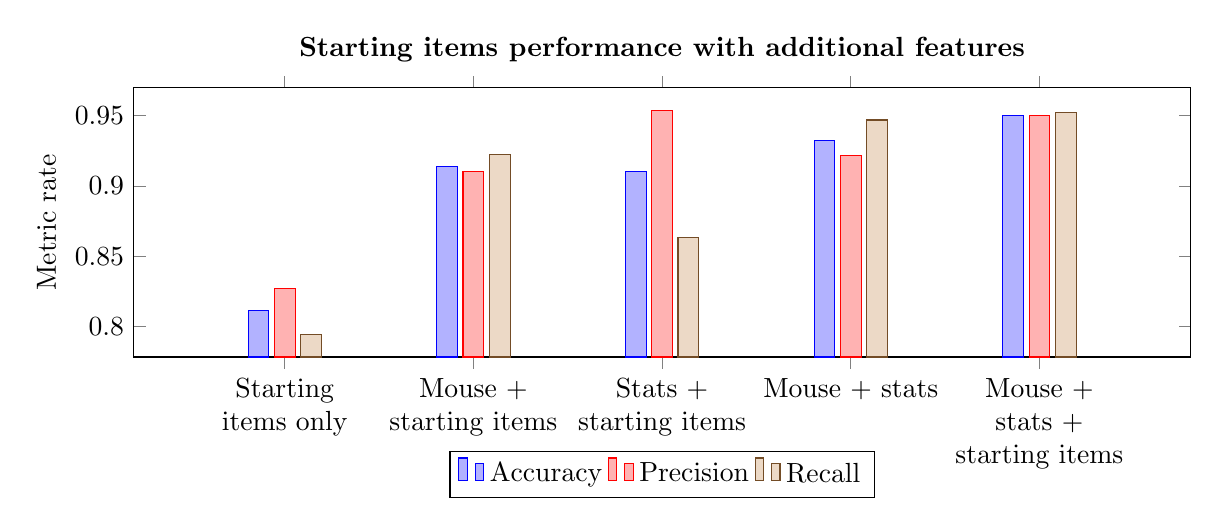
\begin{tikzpicture}
\begin{axis}[
    ybar,
    title={\textbf{Starting items performance with additional features}},
    width=15cm,
    height=5cm,
    %ymin=0.4, ymax=1,
    bar width=0.75em,
    legend style={at={(0.5,-0.35)},anchor=north,legend columns=-1},
    enlarge x limits=0.2,
    x tick label style={align=center,text width=2.5cm},
    symbolic x coords={Starting items only, Mouse + starting items, Stats + starting items, Mouse + stats, Mouse + stats + starting items},
    xtick=data,
    ylabel={Metric rate},
    %cycle list name=exotic,
    %every axis plot/.append style={fill,draw=none,no markers}% <- added
]
\addplot table [x=features, y=accuracy, col sep=comma] {
numSplits,split,accuracy,precision,recall,model,features
1,1,0.811532212460573,0.8271052919831957,0.7941936184067723,Random Forest,Starting items only
1,1,0.9135779793479282,0.9102883801009354,0.9225173648795313,Random Forest,Mouse + starting items
1,1,0.9102086605455826,0.9537679752573119,0.8635228999348816,Random Forest,Stats + starting items
1,1,0.950077781845275,0.9502363396489525,0.9520675059691772,Random Forest,Mouse + stats + starting items
1,1,0.9322103786068515,0.9219059921138925,0.9469068808335143,Random Forest,Mouse + stats

};
\addlegendentry{Accuracy}

\addplot table [x=features, y=precision, col sep=comma] {
numSplits,split,accuracy,precision,recall,model,features
1,1,0.811532212460573,0.8271052919831957,0.7941936184067723,Random Forest,Starting items only
1,1,0.9135779793479282,0.9102883801009354,0.9225173648795313,Random Forest,Mouse + starting items
1,1,0.9102086605455826,0.9537679752573119,0.8635228999348816,Random Forest,Stats + starting items
1,1,0.950077781845275,0.9502363396489525,0.9520675059691772,Random Forest,Mouse + stats + starting items
1,1,0.9322103786068515,0.9219059921138925,0.9469068808335143,Random Forest,Mouse + stats
};
\addlegendentry{Precision}

\addplot table [x=features, y=recall, col sep=comma] {
numSplits,split,accuracy,precision,recall,model,features
1,1,0.811532212460573,0.8271052919831957,0.7941936184067723,Random Forest,Starting items only
1,1,0.9135779793479282,0.9102883801009354,0.9225173648795313,Random Forest,Mouse + starting items
1,1,0.9102086605455826,0.9537679752573119,0.8635228999348816,Random Forest,Stats + starting items
1,1,0.950077781845275,0.9502363396489525,0.9520675059691772,Random Forest,Mouse + stats + starting items
1,1,0.9322103786068515,0.9219059921138925,0.9469068808335143,Random Forest,Mouse + stats
};
\addlegendentry{Recall}

\end{axis}
\end{tikzpicture}
\caption{Performance changes as different features are combined for the random forest classifier.}
\end{figure}

In the first example, an interesting trend occurs when the mouse movement or game statistic features are added to the boots only features for evaluation. The accuracy for the three combinations of features (boots only, mouse movement + boots and game statistics + boots) remain relatively similar, but the precision and recall scores do not. The addition of either mouse movement or game statistics improves the precision of the model while losing recall. There is a shift in predictions, with more false negatives predicted and less false positives. This suggests the model predicts negatives more often, so the addition of mouse movement or statistic data makes two matches look more like they are from different players than without the additional data. This is a form of noise that can be beneficial in some cases. Because the precision is much higher, one can be more confident that when the model predicts two matches are from the same player. If put into a real system, the low false positives would mean players are more unlikely to be falsely accused, but more offenders would go undetected due to the higher number of false negatives. Finally, the combination of all three featuresets together gave the best results, as the recall improved greatly, which improved the accuracy. This contrasts with the results from the previous classification task, where combinations of features generally led to worse performance by adding noise. 

The second example shows a slightly different pattern, where only the combination of statistics and the itemisation features led to high precision and low recall. The combination of mouse movement and itemisation gained a straightforward 10\% increase in prediction performance, which shows the difference between the two itemisation methods, even though using starting items alone performed worse than using boots items alone. The trend of improvement with more features continues and it is also interesting to see that the two encoding methods performed differently alone, but similarly when combined with the other features. Neither improved the model by much when compared to using mouse movements and game statistics, but there were minor improvements, which show the features do not introduce other noise. This leads to the possibility that continually adding more features, though there are diminishing returns can continue to improve prediction rates. 

\subsubsection{Multi-layer perceptron}

Lastly, the combination of features of the neural network model is explored. The combination of the hashed method of encoding for items and other features is highlighted, as it exhibits a similar behaviour to the one observed in the random forest examples, even though it is a different model and item encoding method.

\begin{figure}[H]
\centering
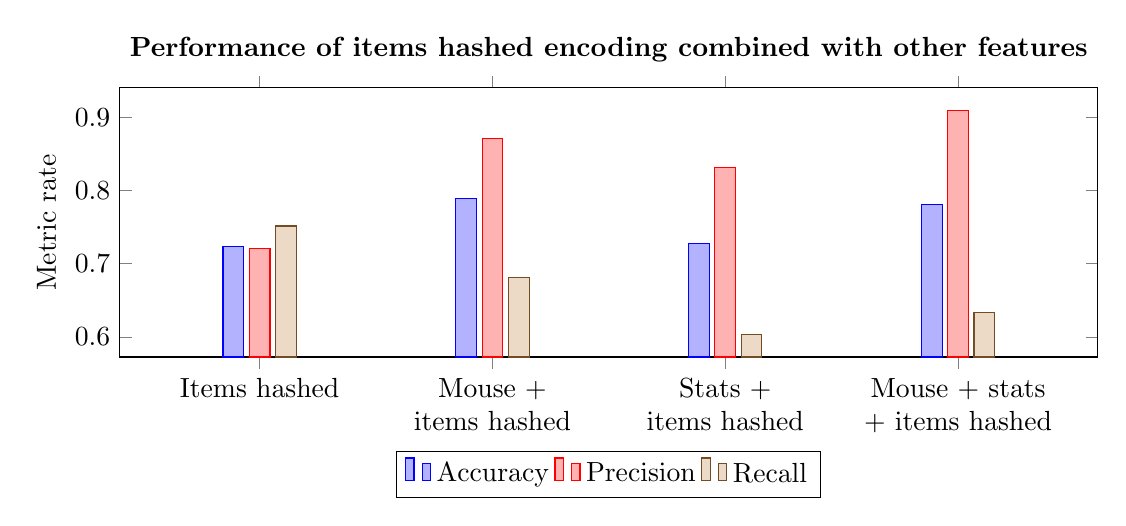
\begin{tikzpicture}
\begin{axis}[
    ybar,
    title={\textbf{Performance of items hashed encoding combined with other features}},
    width=14cm,
    height=5cm,
    %ymin=0.4, ymax=1,
    bar width=0.75em,
    legend style={at={(0.5,-0.35)},anchor=north,legend columns=-1},
    enlarge x limits=0.2,
    x tick label style={align=center,text width=3cm},
    symbolic x coords={Items hashed, Mouse + items hashed, Stats + items hashed, Mouse + stats + items hashed},
    xtick=data,
    ylabel={Metric rate},
    %cycle list name=exotic,
    %every axis plot/.append style={fill,draw=none,no markers}% <- added
]
\addplot table [x=features, y=accuracy, col sep=comma] {
numSplits,split,accuracy,precision,recall,model,features
1,1,0.7236627009084502,0.7208728218636624,0.75156555242023,Multi-layer Perceptron,Items hashed
1,1,0.7888022530904284,0.8715604737666227,0.6813626003907098,Multi-layer Perceptron,Mouse + items hashed
1,1,0.7281298901021465,0.8308107761588446,0.6031202517907532,Multi-layer Perceptron,Stats + items hashed
1,1,0.7806148252941022,0.909545040685867,0.6334111135228999,Multi-layer Perceptron,Mouse + stats + items hashed

};
\addlegendentry{Accuracy}

\addplot table [x=features, y=precision, col sep=comma] {
numSplits,split,accuracy,precision,recall,model,features
1,1,0.7236627009084502,0.7208728218636624,0.75156555242023,Multi-layer Perceptron,Items hashed
1,1,0.7888022530904284,0.8715604737666227,0.6813626003907098,Multi-layer Perceptron,Mouse + items hashed
1,1,0.7281298901021465,0.8308107761588446,0.6031202517907532,Multi-layer Perceptron,Stats + items hashed
1,1,0.7806148252941022,0.909545040685867,0.6334111135228999,Multi-layer Perceptron,Mouse + stats + items hashed
};
\addlegendentry{Precision}

\addplot table [x=features, y=recall, col sep=comma] {
numSplits,split,accuracy,precision,recall,model,features
1,1,0.7236627009084502,0.7208728218636624,0.75156555242023,Multi-layer Perceptron,Items hashed
1,1,0.7888022530904284,0.8715604737666227,0.6813626003907098,Multi-layer Perceptron,Mouse + items hashed
1,1,0.7281298901021465,0.8308107761588446,0.6031202517907532,Multi-layer Perceptron,Stats + items hashed
1,1,0.7806148252941022,0.909545040685867,0.6334111135228999,Multi-layer Perceptron,Mouse + stats + items hashed
};
\addlegendentry{Recall}

\end{axis}
\end{tikzpicture}
\caption{The performance changes of different combinations of the hashed encoding of the itemisation feature and other features for the multi-layer perceptron.}
\label{fig:mlp-pair-combined}
\end{figure}

In figure \ref{fig:mlp-pair-combined}, any combination of features with the hashed items feature results in higher precision and lower recall. As before, this means the model is predicting positive results more accurately and negative results less accurately. It is interesting because when the features were used alone, precision and recall were similar, or in the case of game statistics, the recall was perfect while the precision was low. Yet the opposite is true when the features are used together. This shows that as more features are used, it becomes more certain that two games come from the same player though the difference in two players' behaviour if they are different is less obvious. The additional features add more properties that the model can use to predict if two matches come from the same player, so when it does predict a positive result, it is usually true. However, the additional features also add more variance, making it more difficult to distinguish characteristic similarities of the same player against characteristics of different players, which leads to more false negatives. 

%As this trend spans multiple models and features, it is plausible say this is a property of the classification task in general. When looking at two matches to predict whether they belong to the same player or not, using more features will led to more accurate positive results at the cost of less accurate negative results. In some cases, the right combination of 


%\subsection{Different heroes TODO}
% Use same model and features (best ones) , with only hero differ
% hero id 20, 19 and 15

\subsection{Summary}
In summary, the results found in this set of experiments gave very different results from the previous experiment, which highlights their differences. Logistic regression was the worst performing classifier by far, often unable to reach over 50\% correct classifications. This was also highlighted by the item difference feature - the only feature logistic regression performed well on - as it was a simplified feature compared to all the others. The random forest classifier performed the best, getting high accuracy, precision and recall scores for the range of features tested. Additionally, the combination of features in this problem generally improved results. In some cases those improvements came as an increase in precision at the cost of recall, but in other cases all three metrics were improved. 


% logistic regression bad overall
% different portions of game little effect for mouse movement
% random forest best overall
% combination of features is generally good, improving rates

\end{document}

